\begin{problem}{/images/problems/pic.jpg}{Finding the Area}
	In the figure below, the length of each side of the square is 8cm. Find the area of the green part.

\begin{center}
	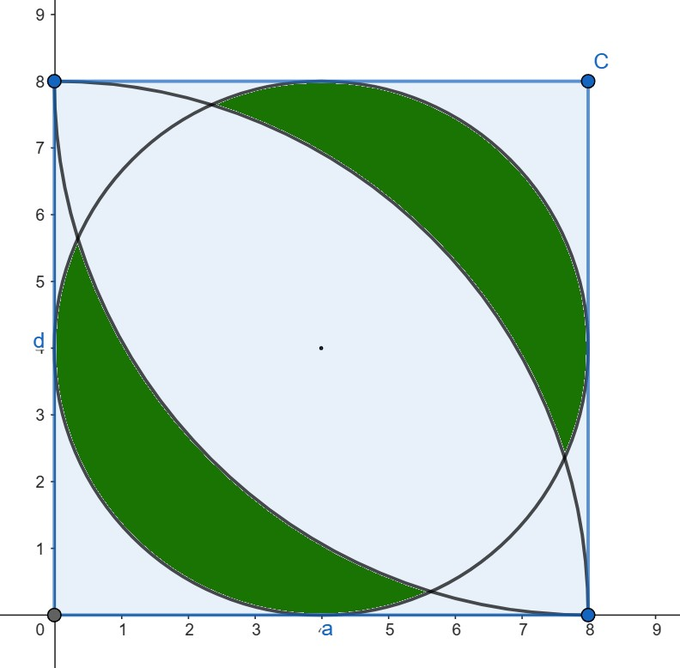
\includegraphics{/images/problems/16_geometry1.jpg}
\end{center}

%(Suggested question from
%[@sina_yari13]( \url{https://twitter.com/sina_yari13)}) ![](/images/problems/16_geometry1.jpg) 
Link to the problem on Twitter: \url{https://twitter.com/Riazi_Cafe/status/1681206384296337408}

\end{problem}
\begin{solution}.
The correct answer is approximately equal to 18.7368.\\[0.2cm]

For simplicity we rotate the image by 45 degrees. Then, using the relationship of the two circles, we define $(x,y)$ as the intersection of the small circle and one of the quarter circles and compute it. Using that, we determine the angles $\alpha \simeq 0.9733$ and $\beta \simeq 2.4188$ defined in the figure below:

\begin{center}
	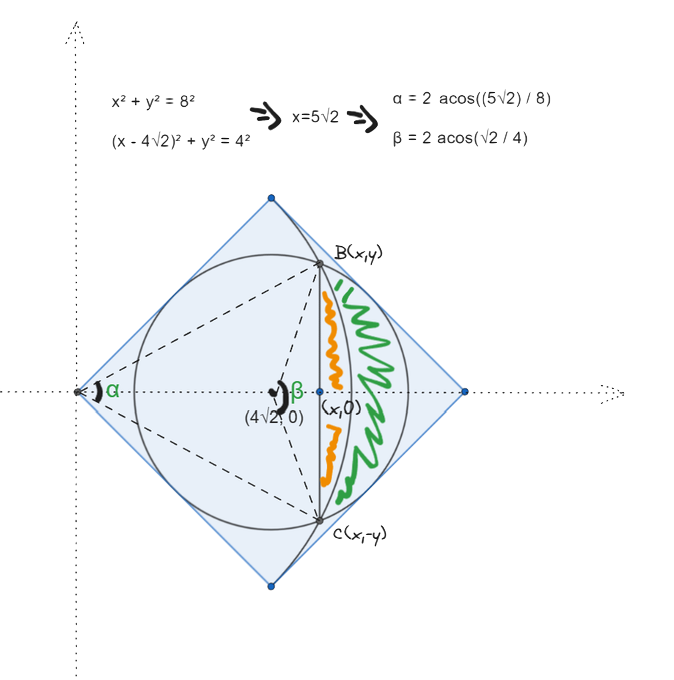
\includegraphics{/images/problems/16_geometry2.jpg}
\end{center}

We then compute the following quantities:
\begin{itemize}
\item The area of the green plus orange parts using $\beta$ and the radius of the smaller circle ($\simeq 14.0593$).
\item The area of the orange part using $\alpha$ and the radius of the quarter circle ($\simeq 4.6909$).
\end{itemize}
Finally, by the latter quantity from the former one, we get the area of each of the green parts ($\simeq 4.6909$). Since we have 2 of these greens parts in the figure, we multiply the answer by 2 to obtain $\simeq 18.7368$.


Link to the solution on Twitter:  \url{https://twitter.com/Riazi_Cafe/status/1681590740441522178}
\end{solution}